%%%%%%%%%%%%%%%%%%%%%%%%%%%%%%%%%%%%%%%%%%%%%%%%%%%%%%%%%%%%%%%%%%%%%%
% problem statement
\begin{statement}[
  problempoints=70,
  timelimit=1 sekunda,
  memorylimit=512 MiB,
]{Lutrija}

\setlength\intextsep{-0.1cm}
\begin{wrapfigure}[7]{r}{0.22\textwidth}
\centering
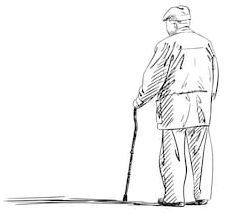
\includegraphics[width=0.22\textwidth]{img/vedran_kurdija.png}
\end{wrapfigure}

Stari Vedran gleda svoju omiljenu emisiju Loto $7/39$ u nadi da će baš on biti
sretnik koji osvaja silne milijune. Loptice skakuću, vrte se i nakon nekog
vremena dio njih izađe iz bubnja. Voditeljica kaže umiljatim glasom: ,,Današnji
brojevi su $2$, $5$, $7$, $11$, $19$, $23$ i $31$. Hvala što ste se igrali s
nama i vidimo se sljedeće srijede!''.

Sav namrgođen jer opet nije pogodio niti jedan broj, Vedran promrlja sebi u
bradu da ne želi više gledati te prostote i krene gasiti televizor. No kako je
Vedran već jako star, nije dobro vidio i umjesto tipke za gašenje pritisnuo je
tipku za promjenu kanala. TV je sada prikazivao HSIN-ov kanal.

Na HSIN-ovom kanalu voditelj je taman pročitao sljedeći zadatak: ,,Dragi
gledatelji, ja ću vam na lijevoj strani ekrana prikazati prosti broj $A$, a na
desnoj prosti broj $B$. Ako mi prvi pošaljete niz prostih brojeva koji počinje
s $A$, a završava s $B$ te je pritom apsolutna razlika između svaka dva susjedna
elementa niza prosti broj, osvojit ćete ulaznicu za Nacionalni park Plitvička
jezera!''

Vedran se sjeća svojih slavnih natjecateljskih dana, no njegova odmakla dob
dala je svoj danak. On nije znao riješiti ovaj zadatak, ali kako vi imate veliko
srce odlučili ste mu pomoći te napisati program koji će riješiti zadani zadatak.

\textbf{Napomena:} prosti broj je prirodan broj veći od $1$ koji je djeljiv samo
s $1$ i sa samim sobom.


%%%%%%%%%%%%%%%%%%%%%%%%%%%%%%%%%%%%%%%%%%%%%%%%%%%%%%%%%%%%%%%%%%%%%%
% Input
\subsection*{Ulazni podaci}
U prvom su retku prosti brojevi $A$ i $B$ $(2 \le A, B \le 10^{14}, A \ne B)$ iz teksta
zadatka.

%%%%%%%%%%%%%%%%%%%%%%%%%%%%%%%%%%%%%%%%%%%%%%%%%%%%%%%%%%%%%%%%%%%%%%
% Output
\subsection*{Izlazni podaci}
Ako je voditelj zadao nemoguć zadatak, u jedini redak ispišite \texttt{-1}.
Inače u prvi redak ispišite broj prostih brojeva u nizu koji je rješenje
zadatka, a u drugi redak ispišite traženi niz iz zadatka. Broj elemenata tog
niza treba biti najviše $10^5$, a svi njegovi elementi trebaju biti manji ili
jednaki $10^{15}$.

Ako postoji više točnih rješenja, ispišite bilo koje.

%%%%%%%%%%%%%%%%%%%%%%%%%%%%%%%%%%%%%%%%%%%%%%%%%%%%%%%%%%%%%%%%%%%%%%
% Scoring
\subsection*{Bodovanje}
U testnim primjerima vrijednima $14$ bodova vrijedit će da, ako postoji rješenje,
postojat će barem jedno u kojem je duljina traženog niza najviše $3$ te će svi
elementi tog niza biti manji ili jednaki $1000$.

U testnim primjerima vrijednima dodatnih $28$ bodova vrijedit će
$2 \le A, B \le 1000$.

%%%%%%%%%%%%%%%%%%%%%%%%%%%%%%%%%%%%%%%%%%%%%%%%%%%%%%%%%%%%%%%%%%%%%%
% Examples
\subsection*{Probni primjeri}
\begin{tabularx}{\textwidth}{X'X'X}
\sampleinputs{test/lutrija.dummy.in.1}{test/lutrija.dummy.out.1} &
\sampleinputs{test/lutrija.dummy.in.2}{test/lutrija.dummy.out.2} &
\sampleinputs{test/lutrija.dummy.in.3}{test/lutrija.dummy.out.3}
\end{tabularx}

%%%%%%%%%%%%%%%%%%%%%%%%%%%%%%%%%%%%%%%%%%%%%%%%%%%%%%%%%%%%%%%%%%%%%%
% We're done
\end{statement}

%%% Local Variables:
%%% mode: latex
%%% mode: flyspell
%%% ispell-local-dictionary: "croatian"
%%% TeX-master: "../hio.tex"
%%% End:
